Nous avons ainsi étudié trois types d'échantillons différents :\\
\begin{itemize}
    \item Le brut, monocristallin, en sortie de fonderie
    \item L'alliage après remise en solution (premier traitement thermique)
    \item L'alliage en fin de traitement, après les deux revenus.\\\\
\end{itemize}



Nous devons donc étudier leur microstructure pour déterminer l'influence des 
différents traitements thermiques sur l'alliage, étant donné que cette microstructure
est le paramètre clé qui va déterminer les propriétés mécaniques de l'alliage,
et notamment sa résistance au fluage.

Étudions tout d'abord les propriétés du brut après fonderie.\\\\


\centerline{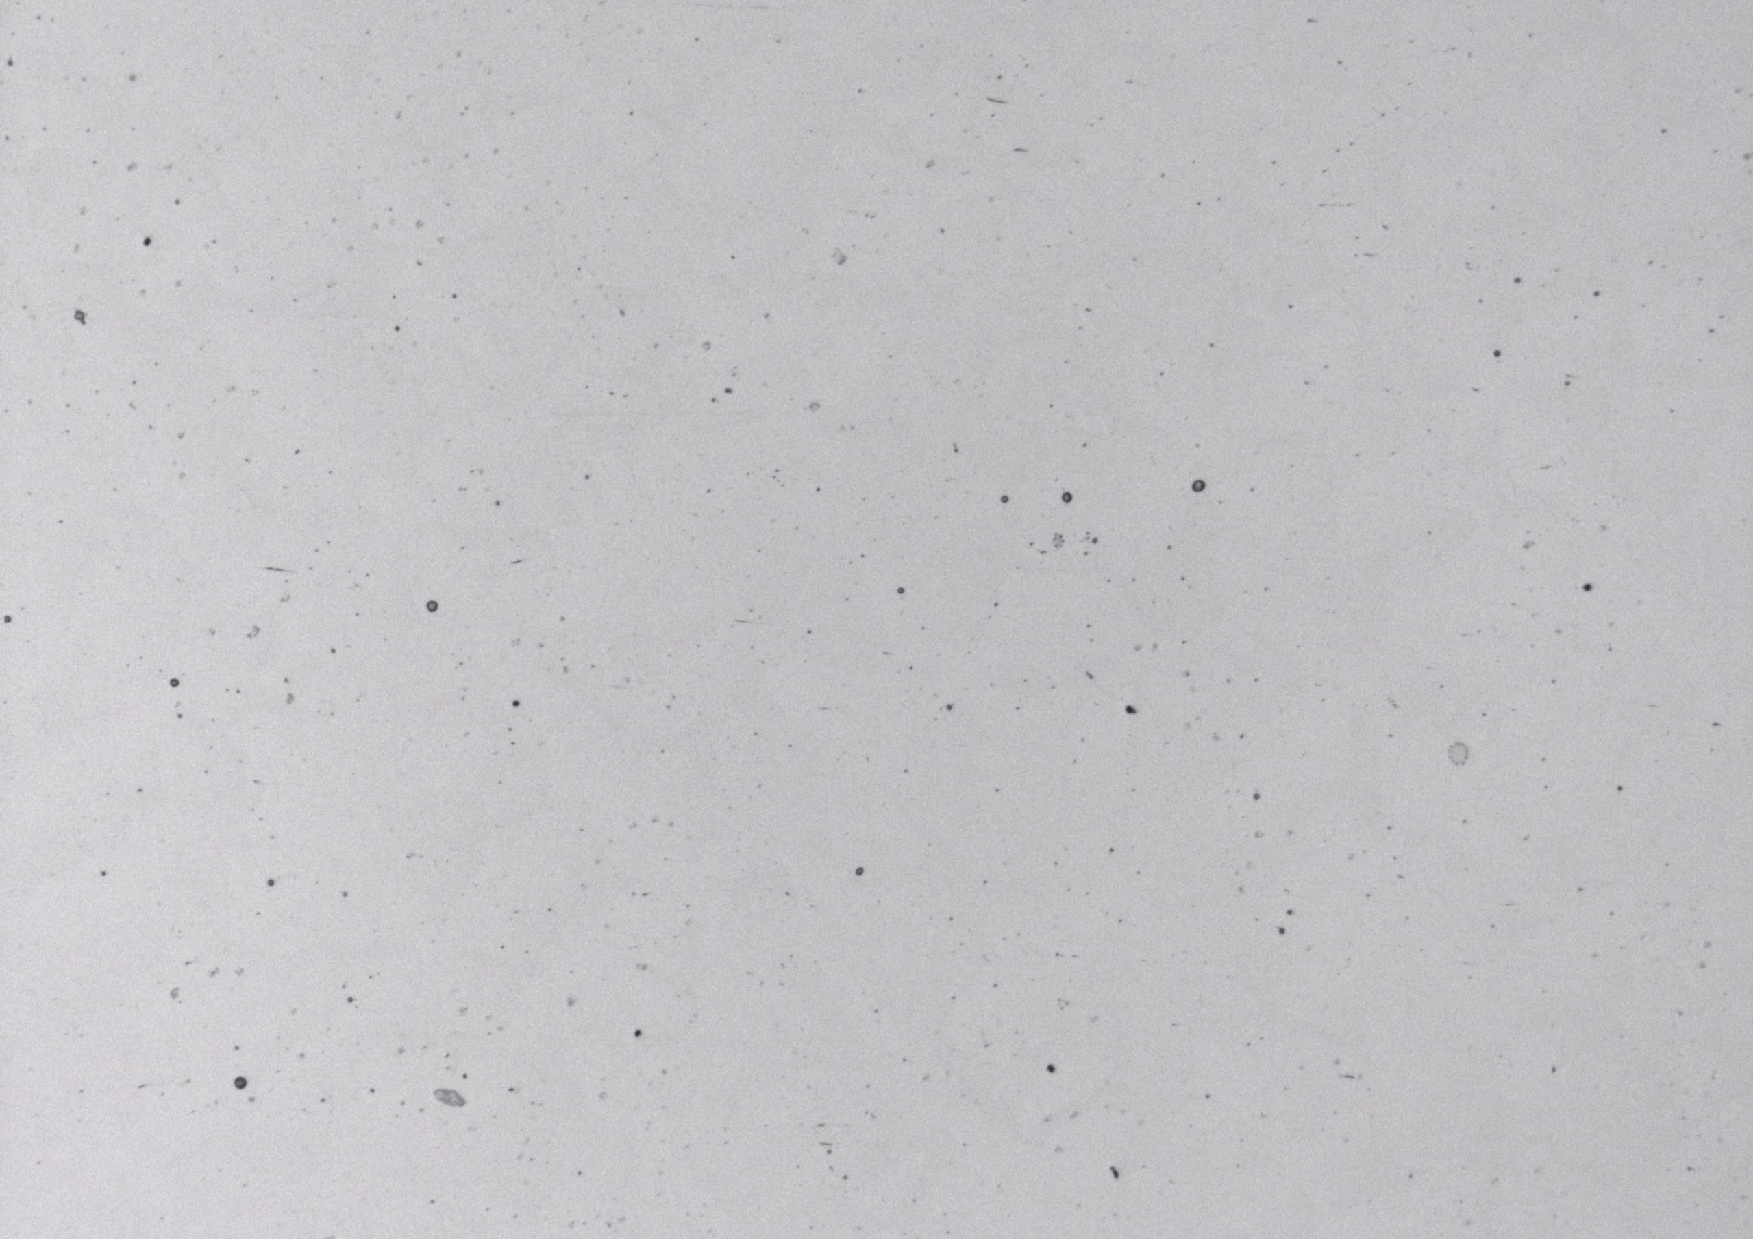
\includegraphics[width=0.75\textwidth]{images_optique/brut.pdf}}
\legend{Le brut de fonderie vu au microscope optique}


Vu au microscope optique, sa surface (après polissage) est lisse
et présente peu de défauts. Cependant, la surface possède 
également de petites tâches noires : ces tâches sont des \emph{pores},
c'est à dire des trous à la surface de l'échantillon. Il y a à ces endroits 
des lacunes importantes dans la maille cristalline, et il manque donc 
une petite portion du matériau. Nous observons également de plus 
petites tâches grises : il s'agit d'agrégats eutectiques, formés lors du refroidissement du liquide.


\centerline{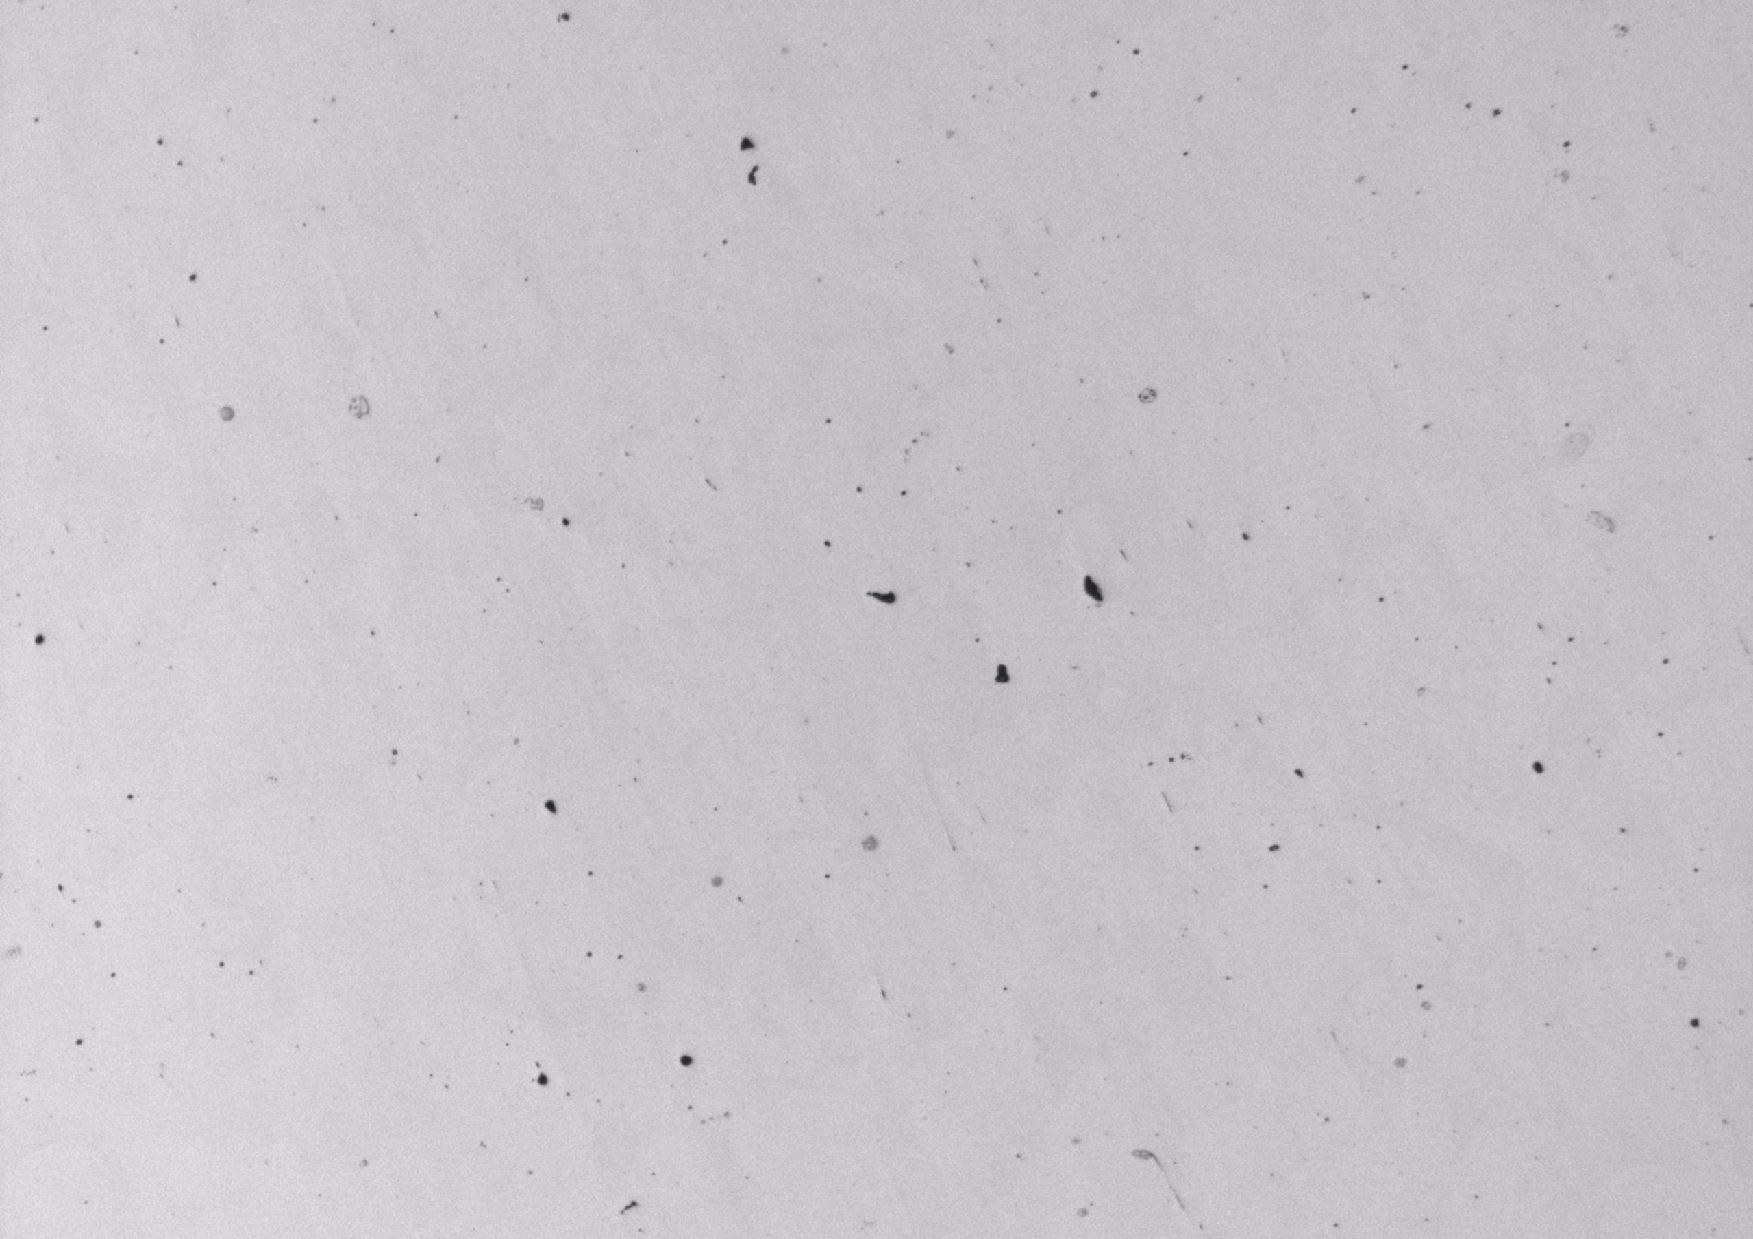
\includegraphics[width=0.75\textwidth]{images_optique/brut2.pdf}}
\legend{Le brut de fonderie vu au microscope optique}

On mesure la proportion de défauts visibles au microscope optique à l'aide du 
logiciel d'analyse d'images ImageJ. Nous obtenons les résultats suivants : \\
\begin{center}
    \begin{tabular}{c|c}
        \textbf{Type de défaut}  & \textbf{Proportion observée}  \\
        \hline
        Pore               & 0,340 \% \\
        Agrégat eutectique & 0,252 \% \\
    \end{tabular}
\end{center}

Nous voyons ainsi une proportion assez nette de défauts au sortir de la fonderie. 
Les agrégats eutectiques apparaissent pendant le refroidissement 
et la solidification du liquide. En effet, la vitesse de refroidissement dans 
la pièce est très difficile à contrôler précisément, et est donc nécessairement
inhomogène.

